\section{Resultados}
\label{sec:resultados}

Tras haber verificado el correcto funcionamiento de cada parte que conforma el proyecto se realizó una implementación del mismo en una placa experimental. En la figura \ref{fig:placa} se puede ver el resultado final de la misma.

\begin{figure}[H]
  \centering
  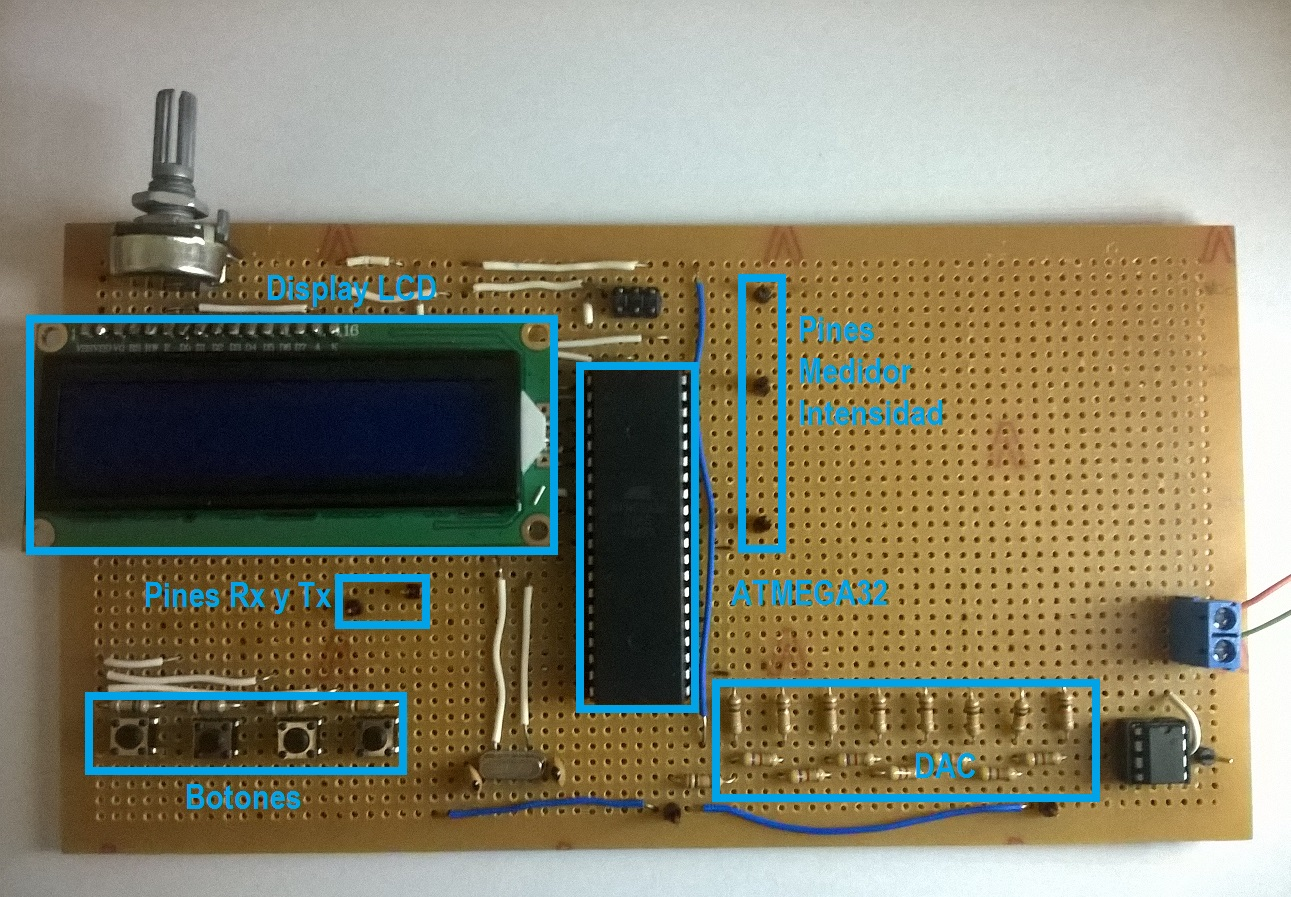
\includegraphics[width=1.0\textwidth]{images/placa.jpg}
  \caption{Versión final del proyecto implementado en una placa experimental.}
  \label{fig:placa}
\end{figure}

Se realizaron mediciones en el osciloscopio de las salidas que se obtienen para las funciones seno y una rampa y en las figuras \ref{fig:salida_rampa} y \ref{fig:salida_seno} se muestran capturas de pantalla del osciloscopio para cada señal.

\begin{figure}[H]
  \centering
  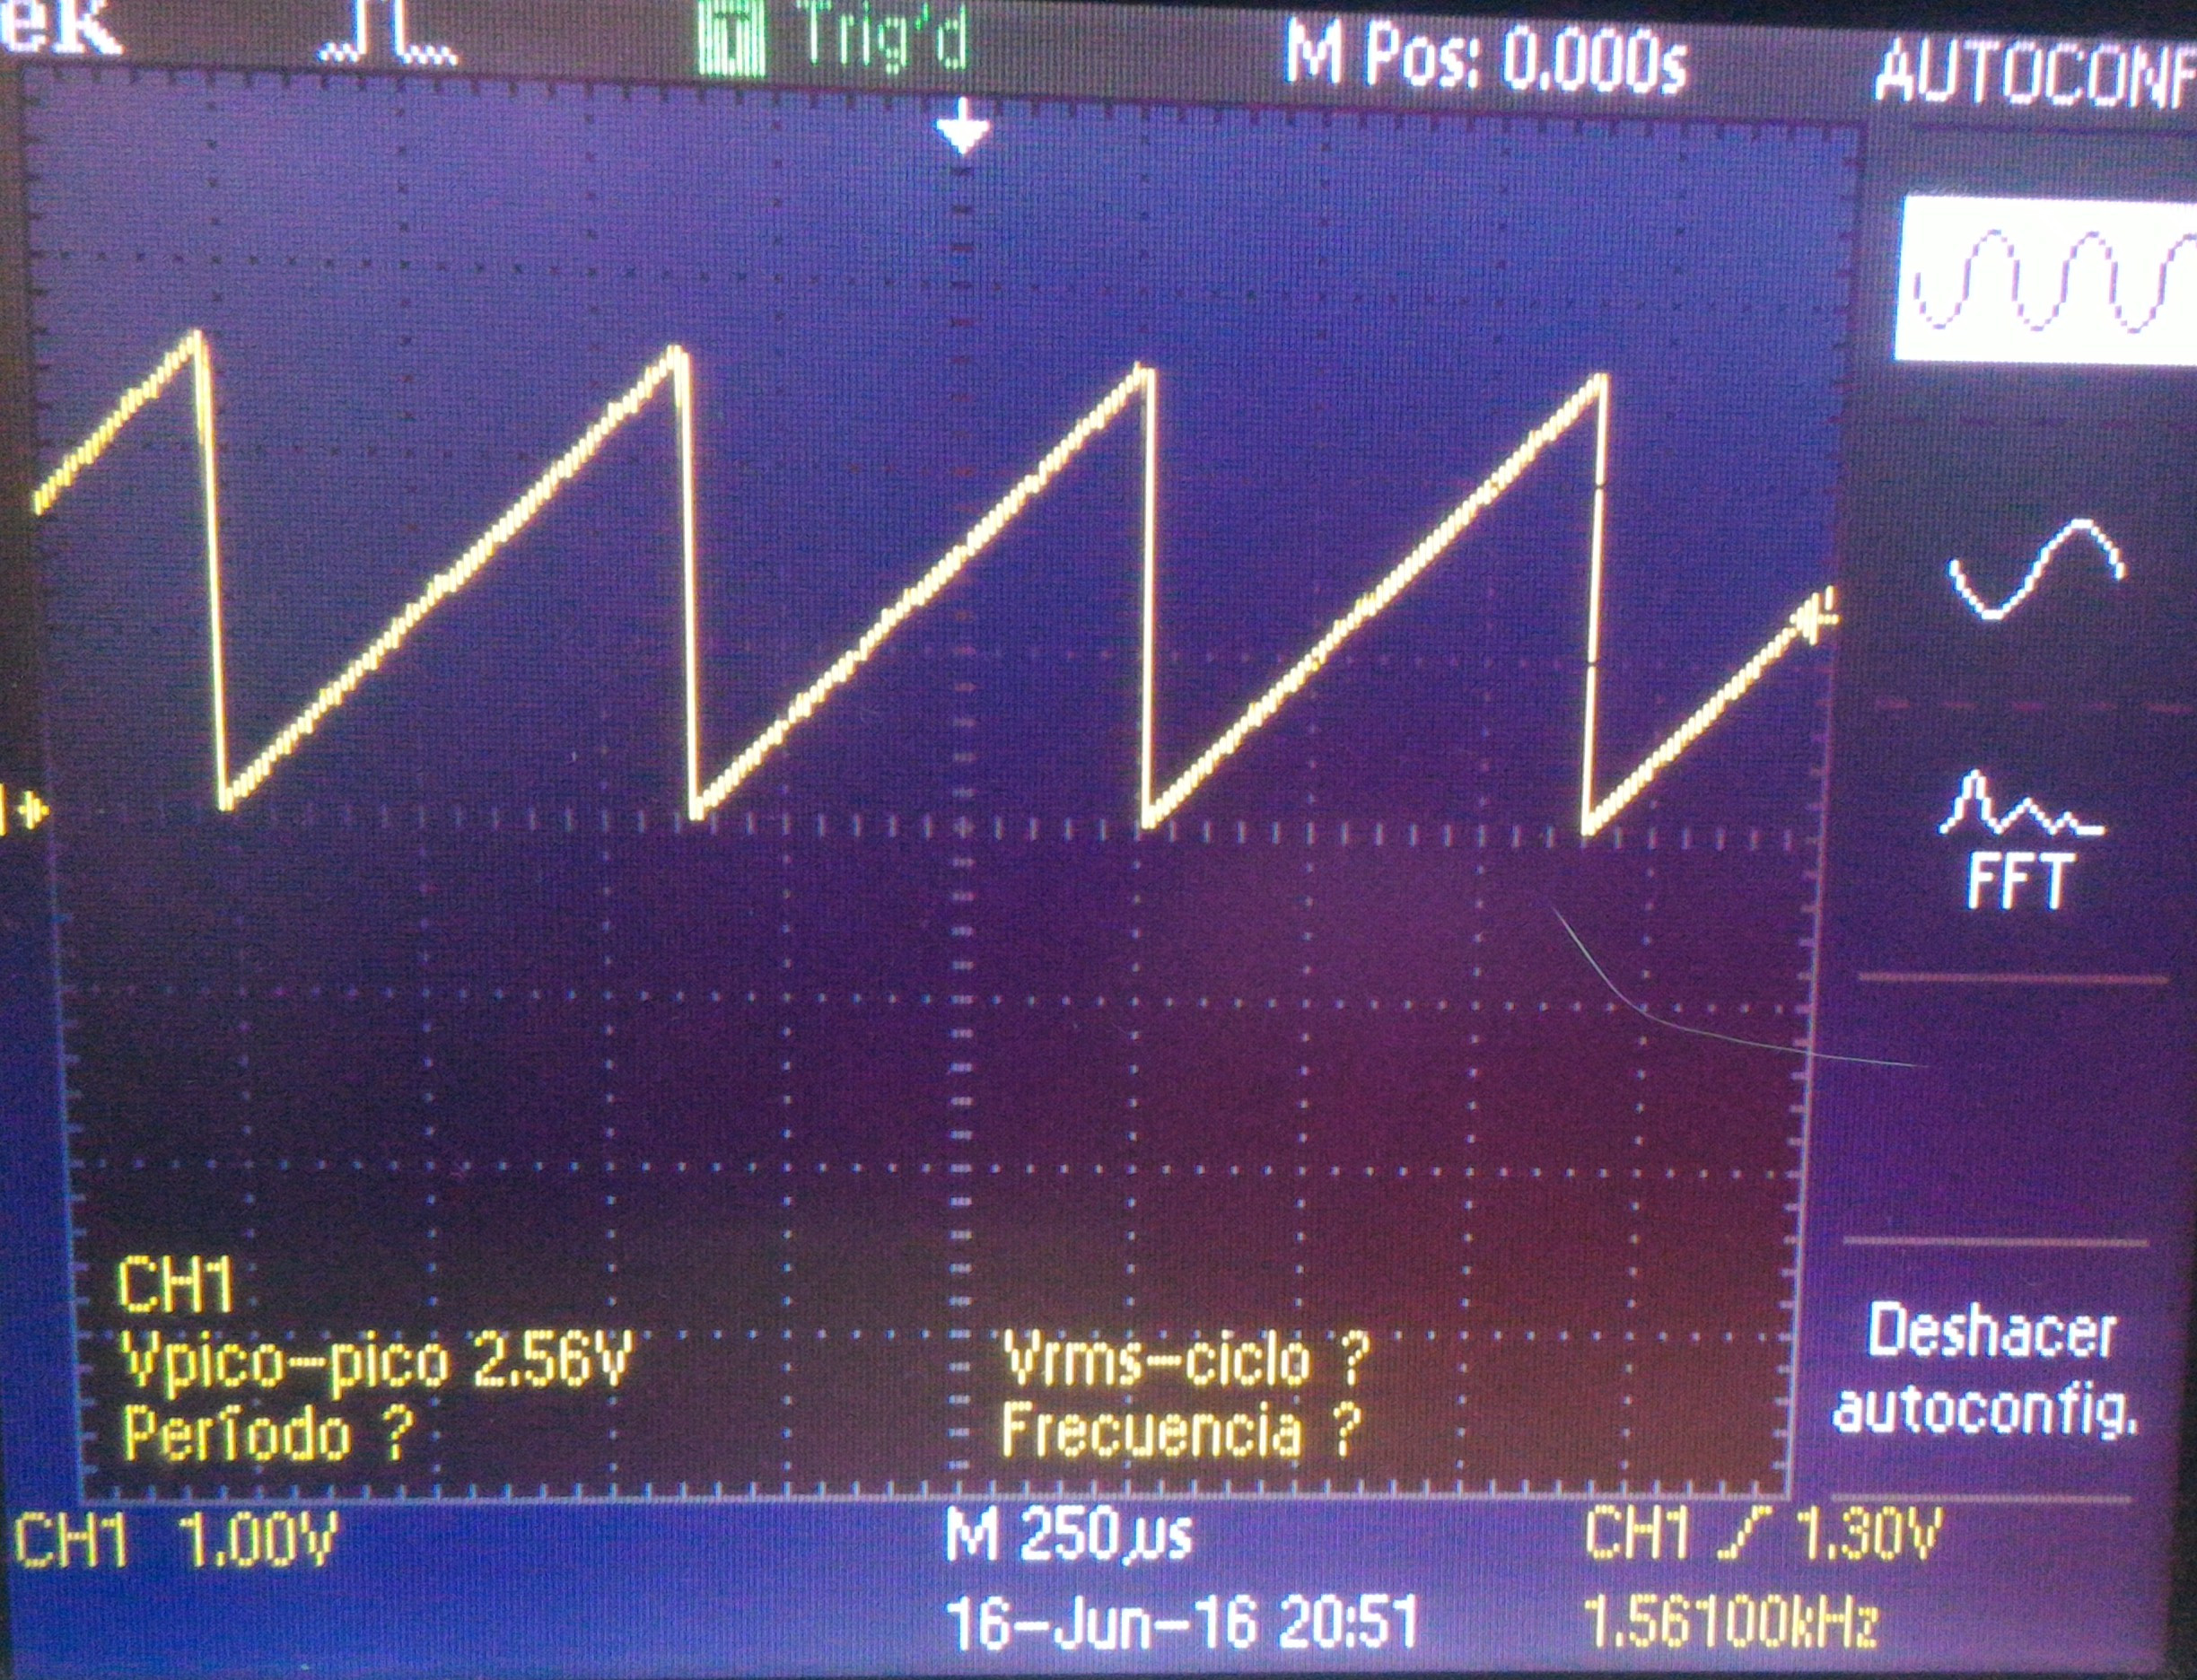
\includegraphics[width=0.8\textwidth]{images/resultados_rampa_precargadav2.jpg}
  \caption{Salida obtenida para la función dientes de sierra/rampa.}
  \label{fig:salida_rampa}
\end{figure}

\begin{figure}[H]
  \centering
  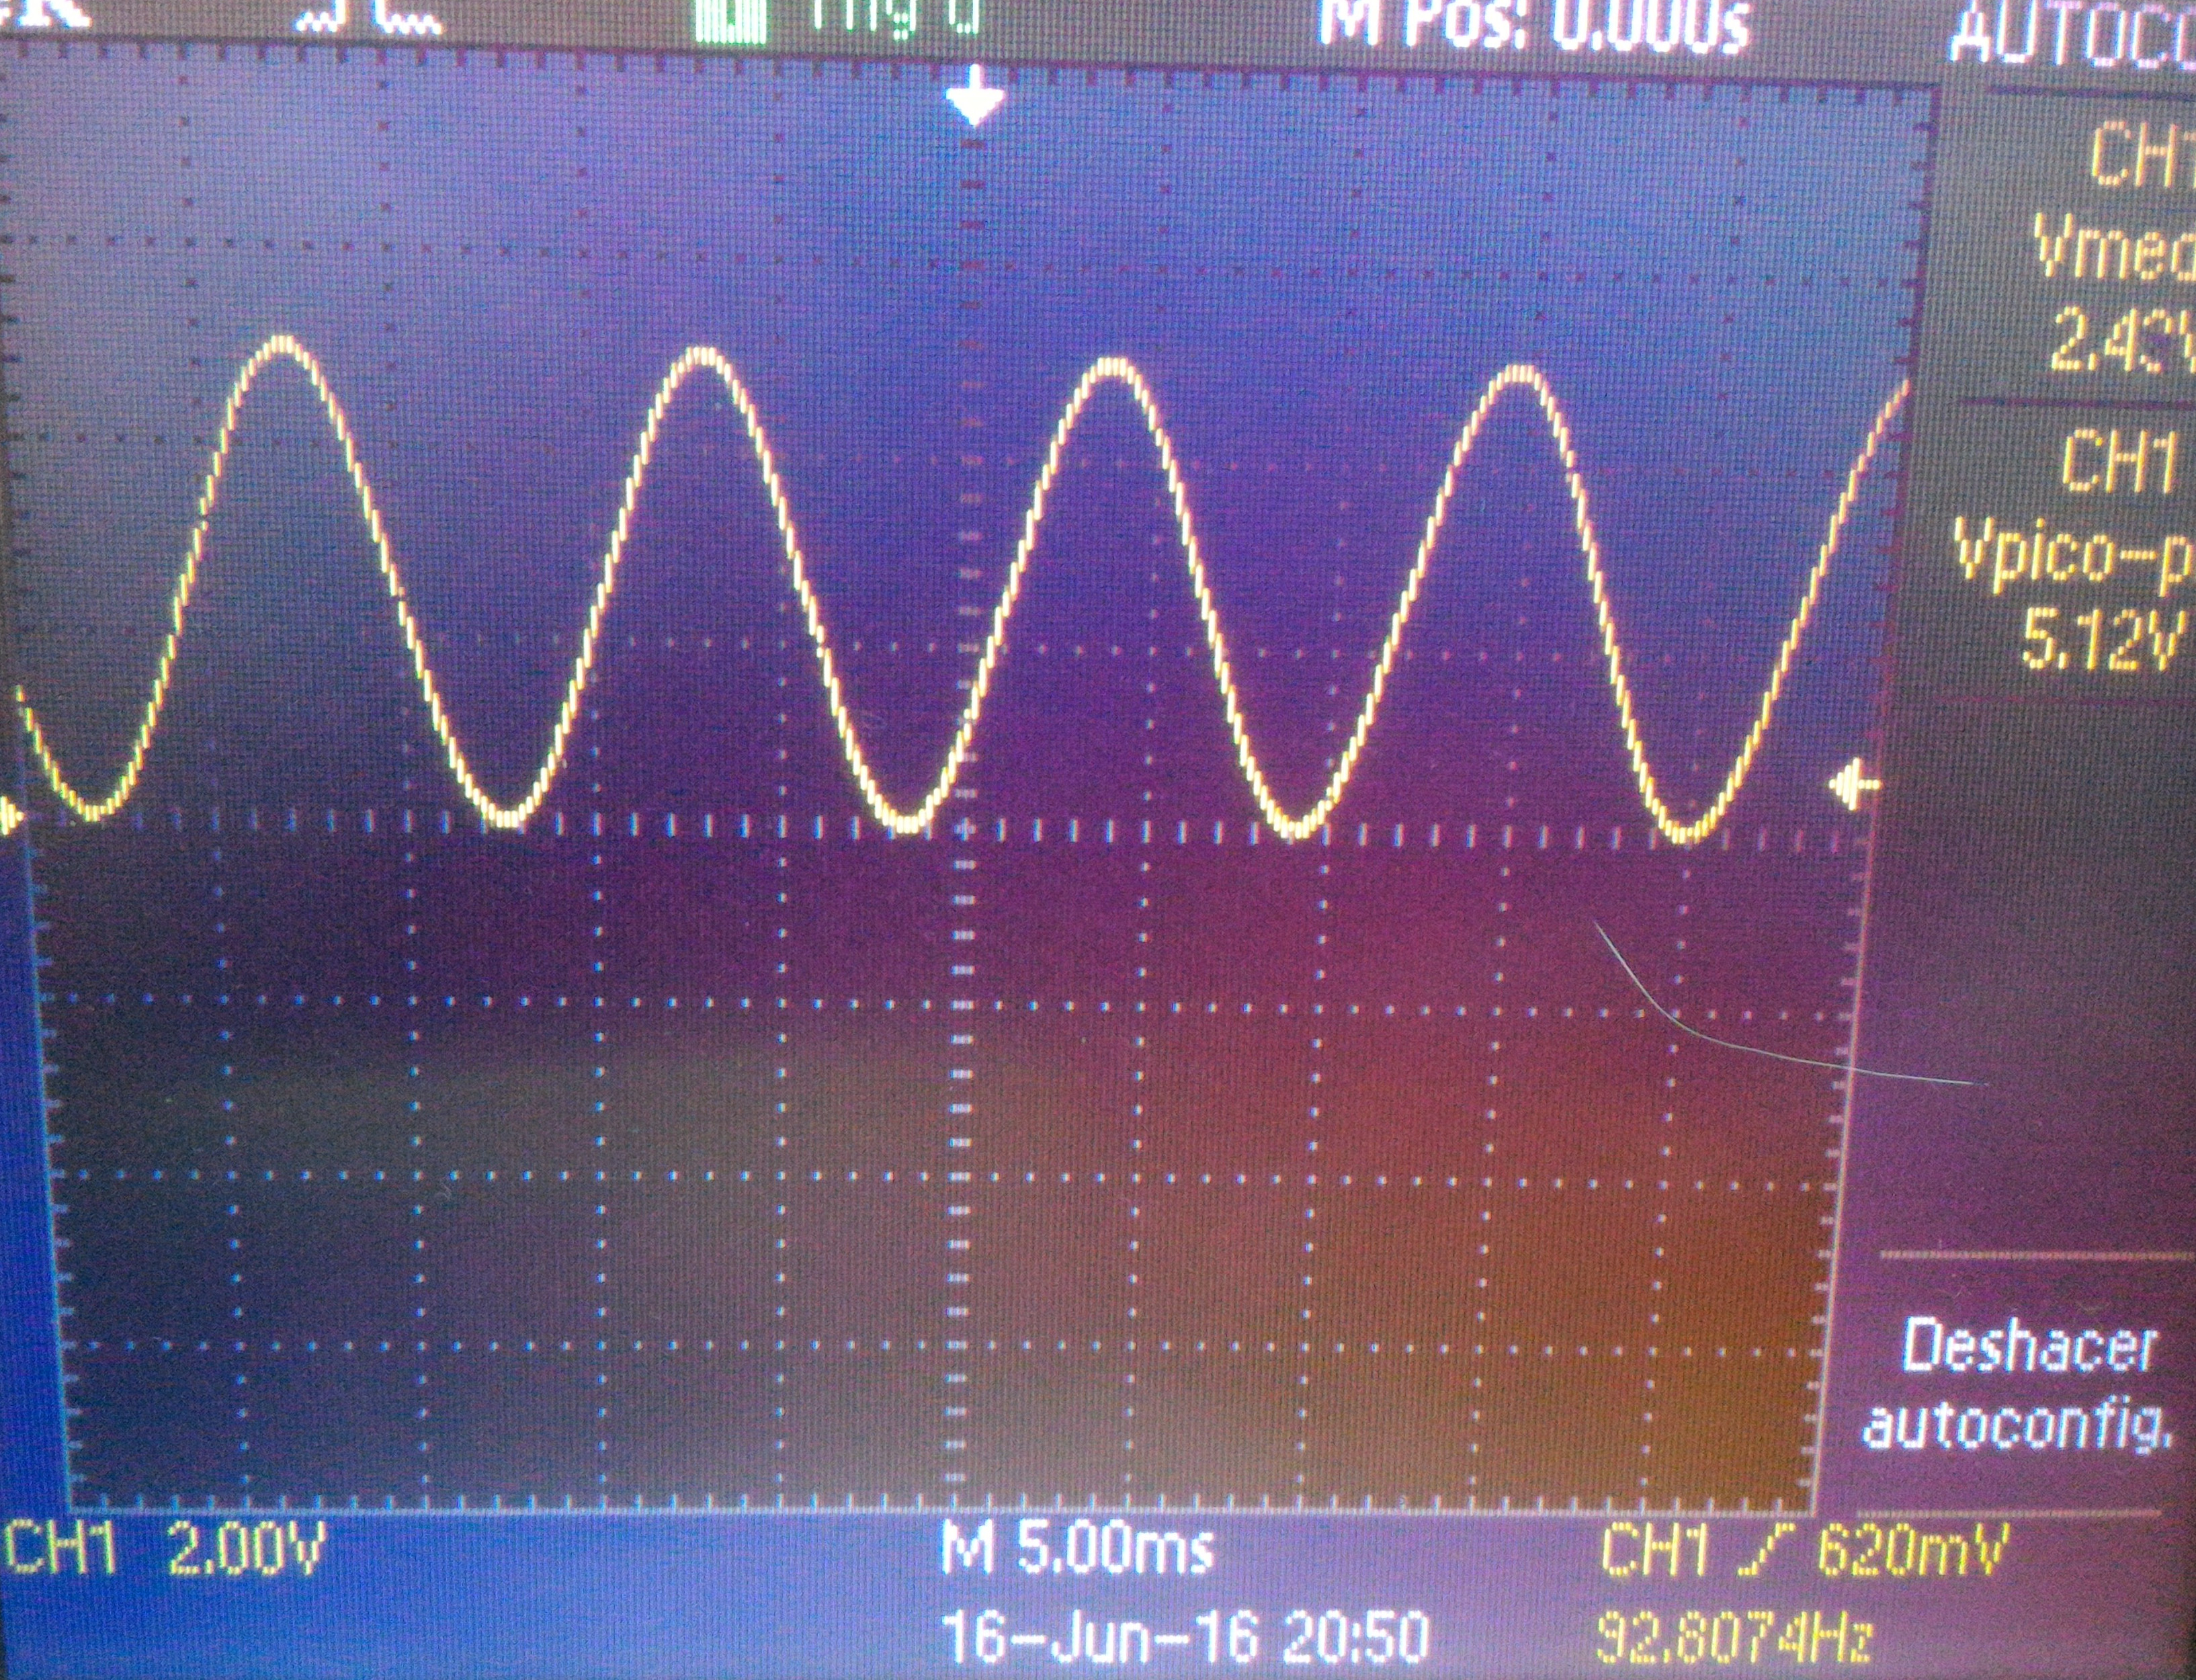
\includegraphics[width=0.8\textwidth]{images/resultados_seno_precargadav2.jpg}
  \caption{Salida obtenida para la función seno.}
  \label{fig:salida_seno}
\end{figure}

En cuanto a los riesgos que se podían presentar que analizamos en el informe de anteproyecto es posible aclarar que el parlante utilizado para poder generar un desplazamiento físico a partir de una señal eléctrica no tuvo problemas de alinealidad y pudo ser incluido en el esquema interferométrico sin mayores problemas. De todas formas, es necesario calibrar la señal de salida para poder obtener resultados óptimos cuando se lo usa en el esquema interferométrico.\\

\begin{figure}[H]
  \centering
  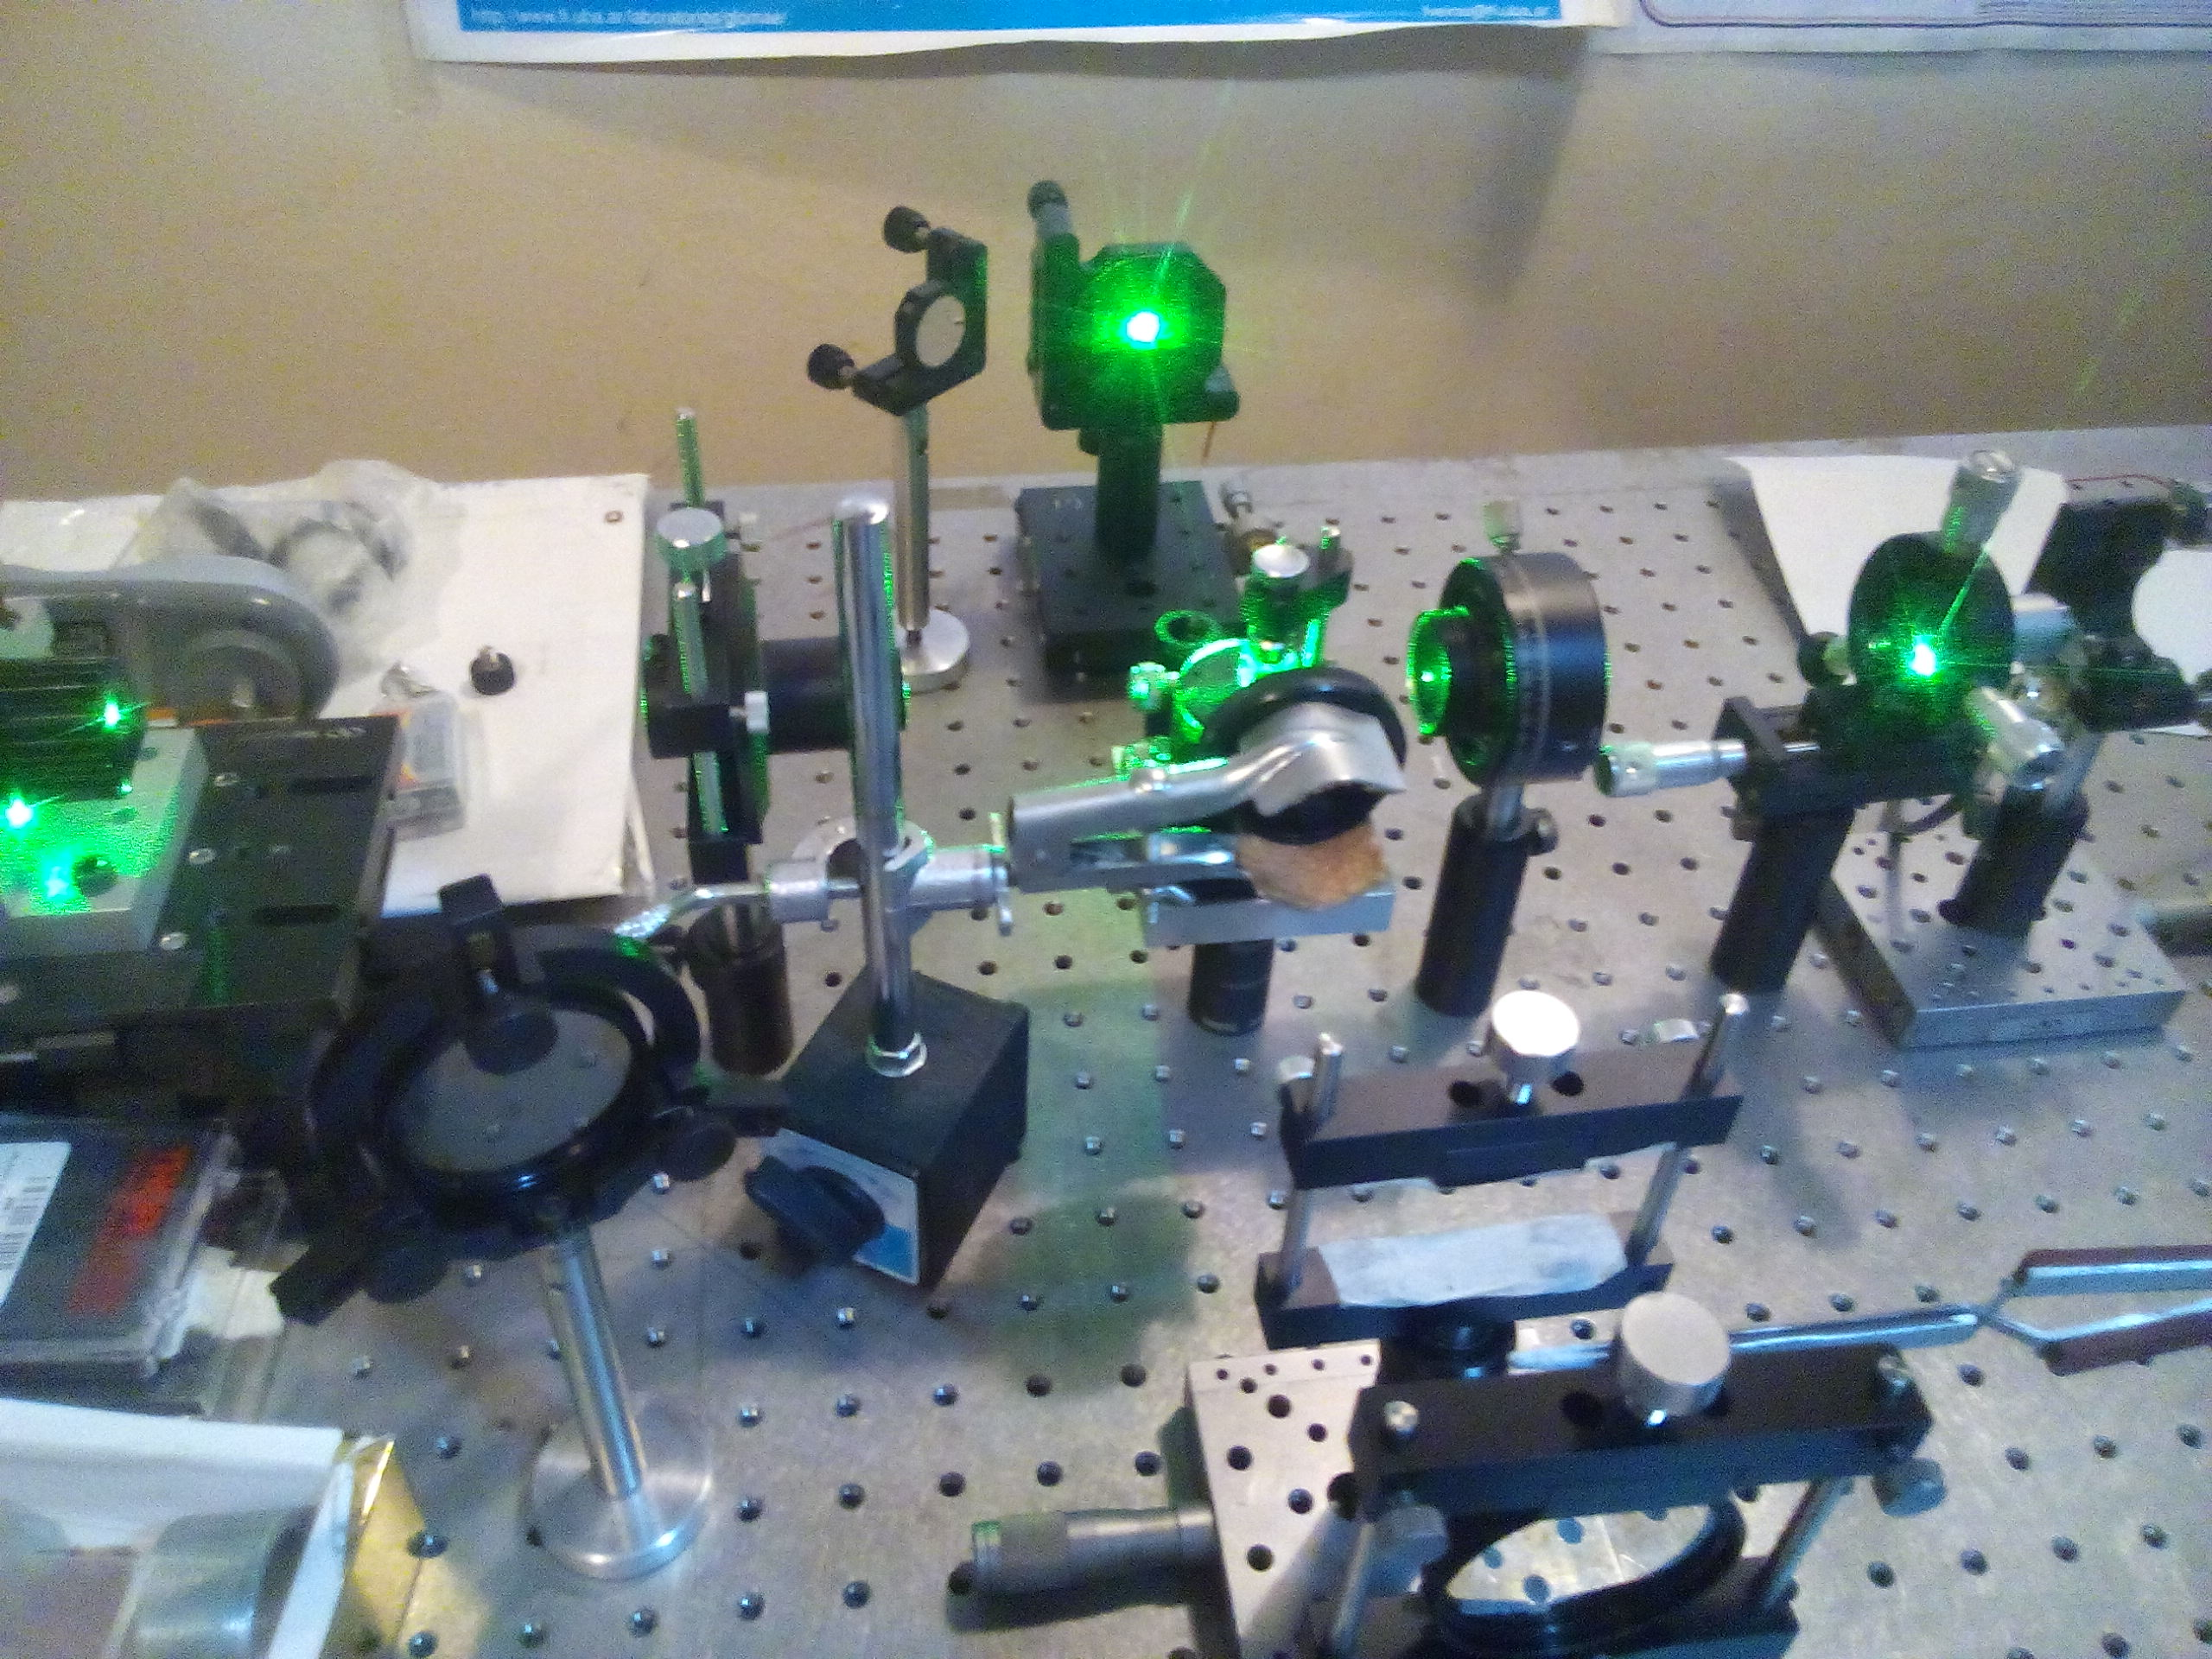
\includegraphics[width=0.8\textwidth]{images/interferometro2.jpg}
  \caption{Interferómetro encendido con el parlante en una de sus ramas}
  \label{fig:interferometro_encendido}
\end{figure}

Por otro lado, otro posible problema era el desarrollo del middleware para pasar las muestras de una señal de Matlab hacia el microcontrolador. Gracias a que Matlab cuenta de antemano con funciones diseñadas para poder comunicarse con un dispositivo serie fue muy sencillo crear un programa que tome muestras de una señal periódica y las envíe al microcontrolador.

Otra de las funciones del proyecto es la medición de intensidad lumínica, se realizaron diversas pruebas sencillas y se verificó el correcto funcionamiento ya que al dejar el módulo de detección completamente a oscuras el valor medido de potencia se vuelve nulo mientras que al utilizar un puntero laser el valor de potencia que se muestra en el display aumenta exponencialmente.

Finalmente, es importante aclarar que si bien es posible verificar el correcto funcionamiento de las diferentes funciones del dispositivo es necesario realizar diferentes experimentos a partir de las cuales va a ser necesario modificar el código del proyecto de manera tal que se logre una precisión mayor que permita que se pueda utilizar en una medición de laboratorio.